% Diapositiva 06
% Kevin

%===========================================
%   4. Explicar la idea general del problema inverso
%   5.Diferenciar problema directo vs problema inverso
%   6.Explicar por qué se usa cálculo multivariado
%===========================================

\begin{frame}{Problema Directo vs Problema Inverso}

    \begin{center}
        \large \textbf{¿Qué información conocemos y qué buscamos?}
    \end{center}
    
    \vspace{0.1cm}
    
    \begin{columns}[T]
    
        %========================================
        % BLOQUE IZQUIERDO
        %========================================
        \column{0.48\textwidth}
        
        \begin{block}{Problema Directo}
            \begin{center}
                % Formalización matemática
                $ \mathbf{m} \longrightarrow \text{Datos} $
                
                \vspace{0.1cm}
                
                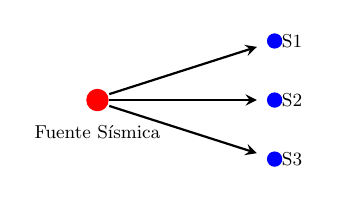
\begin{tikzpicture}[>=stealth, scale=0.75, transform shape]
                    % Fuente
                    \filldraw[red] (0,0) circle (0.18);
                    \node[below] at (0,-0.3) {\small Fuente Sísmica};
                    
                    % Sensores
                    \filldraw[blue] (3,1) circle (0.12);
                    \filldraw[blue] (3,0) circle (0.12);
                    \filldraw[blue] (3,-1) circle (0.12);
                    
                    \node[right] at (3,1) {\small S1};
                    \node[right] at (3,0) {\small S2};
                    \node[right] at (3,-1) {\small S3};
                    
                    % Ondas
                    \draw[->, thick] (0.2,0.1) -- (2.7,0.9);
                    \draw[->, thick] (0.2,0) -- (2.7,0);
                    \draw[->, thick] (0.2,-0.1) -- (2.7,-0.9);
                \end{tikzpicture}
                
                \vspace{0.1cm}
                
                \scriptsize
                Conocemos los parámetros $\mathbf{m} = [x_{\text{real}}, y_{\text{real}}, z_{\text{real}}, A_0]^T$ y calculamos las amplitudes esperadas.
            \end{center}
        \end{block}
    
        %========================================
        % BLOQUE DERECHO
        %========================================
        \column{0.48\textwidth}
        
        \begin{block}{Problema Inverso}
            \begin{center}
                % Formalización matemática
                $ \text{Datos} \longrightarrow \mathbf{m} $
                
                \vspace{0.1cm}
                
                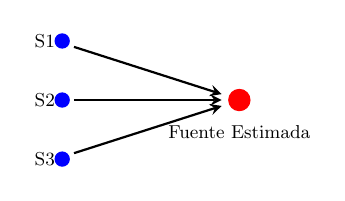
\begin{tikzpicture}[>=stealth, scale=0.75, transform shape]
                    % Sensores
                    \filldraw[blue] (0,1) circle (0.12);
                    \filldraw[blue] (0,0) circle (0.12);
                    \filldraw[blue] (0,-1) circle (0.12);
                    
                    \node[left] at (0,1) {\small S1};
                    \node[left] at (0,0) {\small S2};
                    \node[left] at (0,-1) {\small S3};
                    
                    % Fuente desconocida
                    \filldraw[red] (3,0) circle (0.18);
                    \node[below] at (3,-0.3) {\small Fuente Estimada};
                    
                    % Flechas
                    \draw[->, thick] (0.2,0.9) -- (2.7,0.1);
                    \draw[->, thick] (0.2,0) -- (2.7,0);
                    \draw[->, thick] (0.2,-0.9) -- (2.7,-0.1);
                \end{tikzpicture}
                
                \vspace{0.1cm}
                
                \scriptsize
                A partir de las amplitudes observadas, estimamos el vector de parámetros $\mathbf{m} = [x_{\text{real}}, y_{\text{real}}, z_{\text{real}}, A_0]^T$.
            \end{center}
        \end{block}
    
    \end{columns}
    
    \vspace{0.2cm}
    
    \begin{center}
        \small \textit{“No observamos directamente la fuente; observamos únicamente sus efectos sobre los sensores.”}
    \end{center}
    
\end{frame}